% !TeX encoding = UTF-8
% !TeX program = xelatex
% !TeX spellcheck = en_US

\documentclass[degree=master]{thuthesis}
  % 学位 degree:
  %   doctor | master | bachelor | postdoc
  % 学位类型 degree-type:
  %   academic(默认)| professional
  % 语言 language
  %   chinese(默认)| english
  % 字体库 fontset
  %   windows | mac | fandol | ubuntu
  % 建议终版使用 Windows 平台的字体编译

% 论文基本配置,加载宏包等全局配置
\input{thusetup}
% custom for figures
\usepackage{cuc-custom}

\begin{document}

% 封面
% \maketitle
% 中国传媒大学硕士毕业论文题目

% 学位论文指导小组、公开评阅人和答辩委员会名单
% \input{data/committee}

% 使用授权的说明
% \copyrightpage
% 将签字扫描后授权文件 scan-copyright.pdf 替换原始页面
% \copyrightpage[file=cuc/statement.pdf]
% \includepdf[pages={1}]{cuc/cuc-thesis-cover.pdf}
% 盲审版本封面
\includepdf[pages={1}]{cuc/cuc-thesis-cover-without-name.pdf}
\includepdf[pages={1}]{cuc/statement.pdf}

\frontmatter

\input{data/abstract}

% 目录
\tableofcontents

% 插图和附表清单
% 本科生的插图索引和表格索引需要移至正文之后、参考文献前
\listoffiguresandtables  % 插图和附表清单
% \listoffigures           % 插图清单
% \listoftables            % 附表清单

% help
% include pdf https://stackoverflow.com/questions/2739159/inserting-a-pdf-file-in-latex
% \includepdf[pages=-]{myfile.pdf}
% \includepdf[pages={1}]{myfile.pdf}

% 正文部分
\mainmatter
\ctexset{
  chapter = {
    format      = \sffamily\sanhao,
  },
}
% \titleformat{\chapter}[hang]{\sanhao\heiti}{\thechapter}{1em}{}{\quad\quad}

% 论文一般共六章
% !TeX root = ../main.tex

\chapter{绪论}

我习惯在每章节加一段引入的话,譬如面对XXX带来的挑战,本文提出了一种XXX方法。
本章节就其研究背景、意义、现状以及本文研究内容与组织结构进行简要介绍。


\section{研究背景及意义}

\subsection{研究背景}

一堆乱七八糟的研究背景,加一点宏大叙事。简称懂的都懂。

中国互联网络信息中心(CNNIC) 2021 年 8 月 27 日在京发布的第48次《中国互联网络发展状况统计报告》显示,
% 较2020年12月增长2175万,
截至2021年6月,我国网民规模达10.11亿,
互联网普及率达 71.6\%。
十亿用户接入互联网,形成了全球最为庞大、生机勃勃的数字社会。\cite{cnnic48report}
其中我国网络游戏用户规模达 5.09 亿,占网民整体的 50.4\%。



游戏产业的不断发展,使得游戏的经济属性和文化价值显现得愈加明显,越来越多的人接受了这种集休闲娱乐与文化传播为一体的新兴媒介。
据 Newzoo 2021 全球游戏市场报告\cite{newzoo2021report}表明(如图~\ref{fig:newzoo-player-forecast}),
\begin{figure}[htb]
  \centering
  % 这里可以控制图片宽度比例
  \includegraphics[width=0.8\linewidth]{steins-gate-game-screenshot.jpg}
  \caption{2015-2024年全球玩家数\cite{newzoo2021report}}
  \label{fig:newzoo-player-forecast}
\end{figure}
2021 年全球游戏市场收获近 1758 亿美元,
全球游戏玩家数量将持续增长,到 2023 年将超过三十亿,市场收入也在随之不断增长。
全球三十亿玩家中移动玩家数量约为 28 亿,PC 及主机玩家分别为 14 亿与 9 亿。

...

\subsection{研究意义}

写写研究意义。

% https://www.zhihu.com/question/393670234
关于这个事,我简单说两句,至于我的身份,你明白就行。
总而言之,这个事呢,现在就是这个情况,具体的呢,大家也都看得到,我因为这个身份上的问题,也得出来说那么几句,可能,你听的不是很明白,但是意思就是那么个意思。
我的身份呢,不知道的你也不用去猜,这种事情见得多了,我只想说懂得都懂,不懂的我也不多解释,毕竟自己知道就好,细细品吧。
你们也别来问我怎么了,利益牵扯太大,说了对你我都没好处,当不知道就行了,其余的我只能说这里面水很深,牵扯到很多东西。
详细情况你们自己是很难找的,网上大部分已经删除干净了,所以我只能说懂得都懂。
懂的人已经基本都获利上岸什么的了,不懂的人永远不懂,关键懂的人都是自己悟的,你也不知道谁是懂的人也没法请教,大家都藏着掖着生怕别人知道自己懂事,懂了就能收割不懂的,你甚至都不知道自己不懂。
只是在有些时候,某些人对某些事情不懂装懂,还以为别人不懂。
其实自己才是不懂的,别人懂的够多了,不仅懂,还懂的超越了这个范围,但是某些不懂的人让这个懂的人完全教不懂,所以不懂的人永远不懂,只能不懂装懂。
别人说懂的都懂,只要点点头就行了,其实你懂的我也懂,谁让我们都懂呢,不懂的话也没必要装懂,毕竟里面牵扣扯到很多懂不了的事。
这种事懂的人也没必要访出来,不懂的人看见又来问七问八,最后跟他说了他也不一定能懂,就算懂了以后也对他不好,毕竟懂的太多了不是好事。
所以大家最好是不懂就不要去了解,懂太多不好。

\section{国内外研究现状}

可以分几节来写。
对了一般句子末尾最好不要单独一个字另起一行。

\subsection{论文主要部分的写法}

研究生学位论文撰写,除表达形式上需要符合一定的格式要求外,内容方面上也要遵循一些共性原则。

通常研究生学位论文只能有一个主题(不能是几块工作拼凑在一起),该主题应针对某学科领域中的一个具体问题展开深入、系统的研究,并得出有价值的研究结论。
学位论文的研究主题切忌过大,例如,“中国国有企业改制问题研究”这样的研究主题过大,因为“国企改制”涉及的问题范围太广,很难在一本研究生学位论文中完全研究透彻。

\subsection{论文的语言及表述}

除国际研究生外,学位论文一律须用汉语书写。
学位论文应当用规范汉字进行撰写,除古汉语研究中涉及的古文字和参考文献中引用的外文文献之外,均采用简体汉字撰写。

国际研究生一般应以中文或英文书写学位论文,格式要求同上。
论文须用中文封面。

研究生学位论文是学术作品,因此其表述要严谨简明,重点突出,专业常识应简写或不写,做到立论正确、数据可靠、说明透彻、推理严谨、文字凝练、层次分明,避免使用文学性质的或带感情色彩的非学术性语言。

论文中如出现一个非通用性的新名词、新术语或新概念,需随即解释清楚。

\subsection{论文题目的写法}

论文题目应简明扼要地反映论文工作的主要内容,力求精炼、准确,切忌笼统。
论文题目是对研究对象的准确、具体描述,一般要在一定程度上体现研究结论,因此,论文题目不仅应告诉读者这本论文研究了什么问题,更要告诉读者这个研究得出的结论。
例如:“在事实与虚构之间:梅乐、卡彭特、沃尔夫的新闻观”就比“三个美国作家的新闻观研究”更专业、更准确。

\section{本文研究内容}

总结本文研究内容。
本文的主要目的是……

一篇学位论文的引言大致包含如下几个部分:
1、问题的提出;
2、选题背 景及意义;
3、文献综述;
4、研究方法;
5、论文结构安排。
\begin{itemize}
  \item 问题的提出:要清晰地阐述所要研究的问题“是什么”。
  \item 选题背景及意义:论述清楚为什么选择这个题目来研究,即阐述该研究对学科发展的贡献、对国计民生的理论与现实意义等。
  \item 文献综述:对本研究主题范围内的文献进行详尽的综合述评,“述”的同时一定要有“评”,指出现有研究状态,仍存在哪些尚待解决的问题,讲出自己的研究有哪些探索性内容。
  \item 研究方法:讲清论文所使用的学术研究方法。
  \item 论文结构安排:介绍本论文的写作结构安排。
\end{itemize}

\section{本文组织结构}

本文通过以下六个章节详细论述该研究课题,结构内容如下:

第一章:绪论。本章讨论了XXX以及它所代表的XX方式的意义与可在经济、社会价值上起到的作用,
并回顾国内外现状,明确了本文研究内容与组织结构。

第二章:相关技术概述。本章对后续研究所要使用到的相关技术及概念进行了阐述。文中依次介绍了XXX、XXX、XX与XX等技术的基础原理与作用。...

第三章:XXX。...

第四章:XXX。...

第五章:系统设计与应用。本章从软件工程角度概述了系统的整体设计架构与设计方法,具体介绍了相关开发实现方案与特色功能,将三四章研究内容串联并应用以完成系统开发。
最后对系统进行了展示与测试评估。

第六章:总结与展望。本文目标内容已基本顺利完成,但其研究成果仍然存在许多改进空间。该部分对研究内容与系统成品进行回顾,总结了主旨与存在的问题。
通过思考相应改进措施,对未来研究内容与方向进行展望。

% !TeX root = ../main.tex

\chapter{相关技术概述}

...

本章主要对其中涉及的基本概念与相关技术进行介绍。

\section{西瓜种植}

...
虽然西瓜很好吃,但我不喜欢有很多种子的。

\subsection{西瓜种子的最大公约数}

所以只能边吃西瓜边数种子。
展示一下可以写伪代码,说实话感觉格式优点麻烦。
譬如辗转相除法伪代码示例如下:

\begin{algorithm}
  \caption{辗转相除法}
  \label{alg1}
  \small
  \begin{algorithmic}
    \WHILE{$b \neq 0$}
      \IF{$a \ge b$}
        \STATE $a \leftarrow a - b$
      \ELSE
        \STATE $b \leftarrow b - a$
      \ENDIF
    \ENDWHILE
  \end{algorithmic}
\end{algorithm}




\section{鸡鸭养殖}

鸡鸭适合养在树林里,这样既可以节约空间,鸡也可以找虫子吃,粪便还可作为肥料,旁边要是再有个小池塘就更好了。

\subsection{循环生态的应用}


% TIKZ 画自动机

FSM 逻辑如图~\ref{fig:fsm-logic-example} 所示,它的输入和当前状态决定着下一个状态和输出。

\begin{figure}[htb]
  \centering
  \begin{tikzpicture}[node distance=12pt]
    \node[draw, rounded corners]                        (start)   {输入};
    \node[draw, below right=10pt of start]                         (transition)  {状态转移条件};
    \node[draw, aspect=2, below=60pt of start]     (output conditions)  {输出条件};
    \node[draw, below=of transition]                        (state)  {状态};
    \node[draw, rounded corners, below=of output conditions]  (end)     {输出};
    \coordinate[right=40pt of state] (point1);
    
    \draw[->] (start)  |- (transition);
    \draw[->] (transition) -- (state);
    \draw[->] (state) |-  (output conditions);
    \draw[->] (output conditions) -- (end);
    \draw[->] (start)  -- (output conditions);
    \draw[->] (state)  -- (point1)  |-  (transition);
  \end{tikzpicture}
  \caption{FSM 逻辑示意图} \label{fig:fsm-logic-example}
\end{figure}




\subsection{确定有限状态机}

通常使用没有起点的箭头表示开始状态,双圆圈表示接受状态。
自动机中开始状态也可以是接受状态,此时表示其接受空字符串。

如图 \ref{fig:fsm-binary-even-zero-example} 所示,这是一台用于判断输入二进制字符串是否含有偶数个 0 的有限自动机的逻辑图。
$S_1$ 为开始状态,并代表已经输入了偶数个 0,因此 $S_1$ 也是接受状态。
若输入为不包含 0 或含有偶数个 0 的字符串(例如:1,100,01011等),则自动机以接受状态结束。

\begin{figure}[htb]
  \centering
    \begin{tikzpicture}[shorten >=1pt,auto,transform shape]
    \node[initial,state, accepting] (s1) {$S_1$};
    \node[state] (s2) [right of=s1]  {$S_2$};
    \path[->] (s1) edge [bend left] node [align=center]  {0} (s2)
          (s1) edge [loop above]      node [align=center]  {1} (s1)
          (s2) edge [bend left]       node [align=center]  {0} (s1)
          (s2) edge [loop right]       node [align=center]  {1} (s2);
    \end{tikzpicture}
  \caption{FSM:检测二进制数是否含有偶数个零}
  \label{fig:fsm-binary-even-zero-example}
\end{figure}

同时它也是一个确定有限状态机(DFA),对字母表中每个符号,确定有限自动机的状态都有且仅有一个转移。
它对应的状态转移表如表~\ref{tab:fsm-state-example} 所示:

\begin{table}
  \centering
  \caption{状态转移表}
  \begin{tabular}{c|ccc}
    \toprule
    输入状态 & 1 & 0   \\
    \midrule
    $S_1$   & $S_1$ & $S_2$  \\
    $S_2$   & $S_2$ & $S_1$  \\
    \bottomrule
  \end{tabular}
  \label{tab:fsm-state-example}
\end{table}


\section{虚拟世界}

...

\subsection{坐标系}

还可以用 TIKZ 画坐标系。

目前工业界的各类软件采用坐标系也各不相同,
譬如 Unreal、Unity、Babylon、DirectX 均采用左手坐标系(如图~\ref{fig:left-hand-coordinate-system}),
而 Three.js、Cocos、OpenGL、Vulkan 等则采用右手坐标系(如图~\ref{fig:right-hand-coordinate-system})。

\begin{figure}[htb]
  \centering
  \begin{minipage}[t]{.4\textwidth}
    \centering
    \begin{tikzpicture}[x=0.5cm, y=0.5cm, z=0.3cm]
      % Axes
      \draw [->] (0,0,0) -- (4,0,0) node [at end, right] {$X$};
      \draw [->] (0,0,0) -- (0,4,0) node [at end, left] {$Y$};
      \draw [->] (0,0,0) -- (0,0,4) node [at end, left] {$Z$};
    \end{tikzpicture}
    \caption{左手坐标系}
    \label{fig:left-hand-coordinate-system}
  \end{minipage}
  \begin{minipage}[t]{.4\textwidth}
    \centering
    \begin{tikzpicture}[x=0.5cm, y=0.5cm, z=-0.3cm]
      % Axes
      \draw [->] (0,0,0) -- (4,0,0) node [at end, right] {$X$};
      \draw [->] (0,0,0) -- (0,4,0) node [at end, left] {$Y$};
      \draw [->] (0,0,0) -- (0,0,4) node [at end, left] {$Z$};
    \end{tikzpicture}
    \caption{右手坐标系}
    \label{fig:right-hand-coordinate-system}
  \end{minipage}
\end{figure}


\section{数学公式}

\subsection{四元数的定义}

譬如四元数:

\begin{equation}
  i^2 = j^2 = k^2 = -1 \\
\end{equation}
\begin{equation}
\begin{aligned}
  ij = -ji = k \\
  ki = -ik = j \\
  jk = -kj = i
\end{aligned}
\end{equation}


\subsection{四元数的几何意义}

TIKZ 画坐标系。

在平面坐标系上,以横坐标 R 代表实部,纵坐标 I 代表虚部,复数的几何意义如图~\ref{fig:complex-number}。

\begin{figure}[htb]
  \centering
    \begin{tikzpicture}
      \coordinate (origin) at (0,0);
      \coordinate (ab) at (2,1);
      \coordinate (ba) at (-1,2);

      \draw[-stealth] (-2.5,0) -- (2.5,0) node[right](r) {$R$}; 
      \draw[-stealth] (0,-1) -- (0,2.5) node[right](i) {$I$}; 

      \draw [->, thick] (origin) -- (ab) node[at end, right]{$a+bi$};
      \draw [->, thick] (origin) -- (ba) node[at end, left]{$-b+ai$};
      
      \draw [loosely dashed] (0,1) node[left]{$bi$} -- (ab);
      \draw [loosely dashed] (2,0) node[below]{$a$} -- (ab);

      \draw [loosely dashed] (-1,0) node[below]{$-b$} -- (ba);
      \draw [loosely dashed] (0,2) node[right]{$ai$} -- (ba);

      \pic [draw, -, "$\theta$",angle radius=4pt , angle eccentricity=2] {right angle = ab--origin--ba};
      \pic [draw=red, ->, angle radius=2.23cm, angle eccentricity=2] {angle = ab--origin--ba};
    \end{tikzpicture}
  \caption{复数的几何意义}
  \label{fig:complex-number}
\end{figure}
$(a+bi)*i=-b+ai$,复数乘以 $i$,相当于将平面上复数做逆时针旋转 $\theta$($90^{\circ}$)。

同理非零四元数通常可用于描述三维空间的拉伸与旋转变换,单位 $i$、$j$、$k$ 的几何意义则可以理解为三维空间的一种旋转。
以右手坐标系(如图~\ref{fig:right-hand-coordinate-system})为例,
其中 $i$ 代表绕 $Z$ 轴($X$正向向$Y$轴正向)旋转,$j$ 代表绕 $Y$ 轴($Z$正向向$X$轴正向)旋转,$k$ 代表绕 $X$ 轴($Y$正向向$Z$轴正向)旋转。

四元数模长定义如公式\eqref{eq:quaternion-norm},当 $q=a+bi+cj+dk$,$||q||=1$ 时,它所代表的变换并不会对原向量进行缩放,而是一个纯旋转。
\begin{equation}
  ||q|| = a^2 + b^2 + c^2 + d^2
  \label{eq:quaternion-norm}
\end{equation}

此时 $q$ 被称为单位四元数,也因此它通常被用于表示三维空间的旋转。
同时四元数在静态坐标系中的代数计算,使其避免了动态欧拉角所造成的万向锁问题。

\subsection{四元数的其他优势}

四元数相比旋转矩阵与欧拉角,除了可以避免万向锁问题,还具有其他方面的优势。
譬如速度更快、占用存储空间小、更易于平滑插值等。

3D 空间中任意一个旋转都能够使用三个四元数相乘的形式进行表达,即 $ R_{q}(p) = qpq^{-1} $,其中 $q$ 为一个单位四元数,$p$ 为一个纯四元数。
$ R_{q} $ 表示一个可以将空间点 $p$ 旋转到空间另一个点 $ R_{q}(p) $ 的一个旋转。

定义一个四元数 $ q=a+bi+cj+dk $ 的共轭为 $ q^* = a - bi -cj -dk $。

设 $ \mathbf{v} = bi+cj+dk $,则 $ q=[s,\mathbf{v}] $,$ q^*=[s,-\mathbf{v}] $,此时:
\begin{equation}
qq* = s^2 + v^2 = ||q||^2
\end{equation}

由于 $q^{-1}=\frac{q^*}{||q||^2} $,若使用单位四元数,则模长($ ||q||^2 $)为 1,故此时:
\begin{equation}
q^{-1} = \frac{q^*}{1} = q^*
\end{equation}

存在 3D 旋转公式,任意向量 $\mathbf{v}$ 沿着以单位向量定义的旋转轴 $\mathbf{u}$ 旋转 $\theta$ 度之后的 $\mathbf{v}^{'}$ 可以使用四元数乘法获得。
令 $v=[0,\mathbf{v}]$,$q=[\cos{\frac{1}{2}\theta},\sin{\frac{1}{2}\theta}\mathbf{u}]$,则:
\begin{equation}
v^{'} = qvq^{-1} = qvq^*
\end{equation}

同时存在与单位四元数旋转效果相同的 3D 旋转矩阵,即任意向量 $\mathbf{v}$ 沿着以单位向量定义的旋转轴 $\mathbf{u}$ 旋转 $\theta$ 角度之后的 $\mathbf{v}^{'}$ 可以使用矩阵乘法来获得。

令 $a=\cos{\frac{1}{2}\theta}$,$b=\sin{\frac{1}{2}\theta}u_x$,$c=\sin{\frac{1}{2}\theta}u_y$,$d=\sin{\frac{1}{2}\theta}u_z$,那么:
\begin{equation}
  \mathbf{v}^{'} = 
  \begin{bmatrix}
    1-2c^2-2d^2 & 2bc-2ad & 2ac+2bd \\
    2bc+2ad & 1-2b^2-2d^2 & 2cd-2ab \\
    2bd-2ac & 2ab+2cd & 1-2b^2-2c^2 \\
  \end{bmatrix}
  \mathbf{v}
\end{equation}

由上可知,四元数相对于旋转矩阵,使用 $q^*$ 替换 $q^{-1}$,大大提高了求四元数的逆的计算效率,同时比旋转矩阵的计算更为快速方便。
此外,四元数对应实部与虚部 $ijk$ 只需要存储四个数值,空间占用也远小于同等效果的旋转矩阵。

\subsubsection{绘制箭头示例}

线性插值(Lerp)会沿一条直线进行插值,如图 \ref{fig:lerp} 所示,$v_t$ 在 $v_0$ 与 $v_1$ 组成的三角形斜边上滑动。

\begin{figure}[htb]
  \centering
  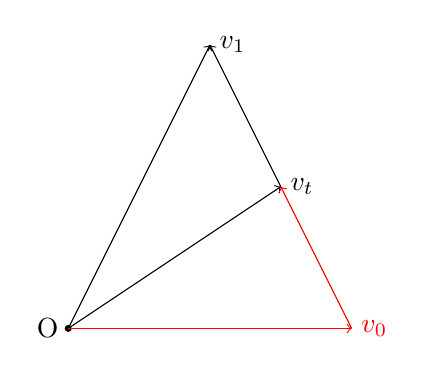
\begin{tikzpicture}[scale=0.9]
    \coordinate (o) at (0,0);
    \coordinate (v1) at (2,4);
    \coordinate (vt) at (3,2);
    \coordinate (v0) at (4,0);
    
    \fill[black] (o) circle (0.05) node[left]{O};
    
    \draw[->] (o) -> (v1) node[right]{$v_1$};
    \draw[->] (o) -> (vt) node[right]{$v_t$};
    \draw[red, ->] (o) -> (v0) node[right]{$v_0$};
    \draw[red, ->] (v0) -> (vt);
    \draw[->] (vt) -> (v1);
  \end{tikzpicture}
  \caption{线性插值示意图}
  \label{fig:lerp}
\end{figure}

$v_t$ 可写为 $v_0 + (v_1-v_0)t$,其中 $t$ 是插值的参数,取值范围为 $[0,1]$。
\begin{equation}
  v_t = Lerp(v_0, v_1,t) = v_0 + (v_1-v_0)t = (1-t)v_0+tv_1
\end{equation}

将 Lerp 应用于单位四元数上,可得:
\begin{equation}
  q_t = Lerp(q_0, q_1, t) = (1-t)q_0 + tq_1
  \label{eq:quaternions-lerp}
\end{equation}

\subsection{贝塞尔曲线}

贝塞尔曲线最初由 Paul de Casteljau 使用 de Casteljau 算法开发,是一种计算曲线的稳定方法。
其根据控制点的数量可分为不同阶,常见类型有线性贝塞尔曲线、二次贝塞尔曲线(也曾被用于 TrueType 的字体平滑)、三次贝塞尔曲线等。

线性贝塞尔曲线等同于线性插值,给定两个控制点 $P_0$ 与 $P_1$,则公式为:
\begin{equation}
  {\mathbf  {B}}(t)={\mathbf  {P}}_{0}+({\mathbf  {P}}_{1}-{\mathbf  {P}}_{0})t=(1-t){\mathbf  {P}}_{0}+t{\mathbf  {P}}_{1}{\mbox{ , }}t\in [0,1]
\end{equation}

二次贝塞尔曲线给定三个点 $P_1$、$P_2$ 与 $P_3$,公式为:
\begin{equation}
  {\mathbf  {B}}(t)=(1-t)^{{2}}{\mathbf  {P}}_{0}+2t(1-t){\mathbf  {P}}_{1}+t^{{2}}{\mathbf  {P}}_{2}{\mbox{ , }}t\in [0,1]
\end{equation}

三次贝塞尔曲线如图~\ref{fig:bezier-curve-3rd} 所示,给定四个点 $P_1$、$P_2$、$P_3$ 与 $P_4$,公式为:
\begin{equation}
  {\mathbf  {B}}(t)={\mathbf  {P}}_{0}(1-t)^{3}+3{\mathbf  {P}}_{1}t(1-t)^{2}+3{\mathbf  {P}}_{2}t^{2}(1-t)+{\mathbf  {P}}_{3}t^{3}{\mbox{ , }}t\in [0,1]
\end{equation}

\begin{figure}[htb]
  \centering
  \begin{tikzpicture}[scale=1.3]
    \coordinate (p0) at (0,0);
    \coordinate (p1) at (2,2);
    \coordinate (p2) at (4,2);
    \coordinate (p3) at (4,0);
    
    \fill[black] (p0) circle (0.05) node[left]{$P_0$};
    \fill[black] (p1) circle (0.05) node[above]{$P_1$};
    \fill[black] (p2) circle (0.05) node[above]{$P_2$};
    \fill[black] (p3) circle (0.05) node[right]{$P_3$};
    
    \draw[dashed] (p0) -> (p1);
    \draw[dashed] (p1) -> (p2);
    \draw[dashed] (p2) -> (p3);
  
    \draw (p0) .. controls (p1) and (p2) .. (p3);
  \end{tikzpicture}
  \caption{三次贝塞尔曲线}
  \label{fig:bezier-curve-3rd}
\end{figure}

$n$ 阶贝塞尔曲线给定 $P_0$、$P_1$、…、$P_n$ 等 $n+1$ 个点,公式可递归表达为:
\begin{equation}
  {\mathbf  {B}}(t)={\mathbf  {B}}_{{{\mathbf  {P}}_{0}{\mathbf  {P}}_{1}\ldots {\mathbf  {P}}_{n}}}(t)=(1-t){\mathbf  {B}}_{{{\mathbf  {P}}_{0}{\mathbf  {P}}_{1}\ldots {\mathbf  {P}}_{{n-1}}}}(t)+t{\mathbf  {B}}_{{{\mathbf  {P}}_{1}{\mathbf  {P}}_{2}\ldots {\mathbf  {P}}_{n}}}(t)
\end{equation}

De Casteljau 算法\cite{farin2000essentials}即基于此公式,采用递归方式来计算一组控制点所构建的贝塞尔曲线所经过的点。

给定 $P_0$ 到 $P_3$ 的控制点,将其分解为 $L_0L_1L_2L_3$ 与 $R_0R_1R_2R_3$ 继续绘制,并可通过级别控制绘制的精细度,
关键点如图~\ref{fig:de-casteljau} 所示:

\begin{figure}[htb]
  \centering
  \begin{tikzpicture}
    \coordinate (p0) at (0,0);
    \coordinate (p1) at (4,4);
    \coordinate (p2) at (8,4);
    \coordinate (p3) at (8,0);
    \coordinate (h) at (6,4);
    \coordinate (l0) at (0,0);
    \coordinate (l1) at (2,2);
    \coordinate (l2) at (4,3);
    \coordinate (l3) at (5.5,3);
    \coordinate (r0) at (5.5,3);
    \coordinate (r1) at (7,3);
    \coordinate (r2) at (8,2);
    \coordinate (r3) at (8,0);
    
    \fill[black] (h) circle (0.05) node[above]{$H$};
    
    \fill[black] (p0) circle (0.05) node[left]{$P_0$};
    \fill[black] (p1) circle (0.05) node[above]{$P_1$};
    \fill[black] (p2) circle (0.05) node[above]{$P_2$};
    \fill[black] (p3) circle (0.05) node[right]{$P_3$};
    
    \fill[black] (l0) circle (0.05) node[right]{$L_0$};
    \fill[black] (l1) circle (0.05) node[above]{$L_1$};
    \fill[black] (l2) circle (0.05) node[above]{$L_2$};
    \fill[black] (l3) circle (0.05) node[below right]{$L_3$};
    
    \fill[black] (r0) circle (0.05) node[below left]{$R_0$};
    \fill[black] (r1) circle (0.05) node[above]{$R_1$};
    \fill[black] (r2) circle (0.05) node[right]{$R_2$};
    \fill[black] (r3) circle (0.05) node[left]{$R_3$};
    
    \draw[-] (p0) -> (p1);
    \draw[-] (p1) -> (p2);
    \draw[-] (p2) -> (p3);
    
    \draw[red] (l1) -> (h);
    \draw[red] (h) -> (r2);
    \draw[blue] (l2) -> (r1);
  
  \end{tikzpicture}
  \caption{De Casteljau 算法绘制过程}
  \label{fig:de-casteljau}
\end{figure}

绘制 $P_0$ 到 $P_3$ 曲线的代码示例如下所示:

\begin{lstlisting}[language=python]
% 返回这两点间线段的中点
def midpoint((x1, y1), (x2, y2)):
    return ((x1+x2)/2, (y1+y2)/2)

% 绘制级别,可决定精细度
MAX_LEVEL = 5
def draw_curve(P0, P1, P2, P3, level=1):
    % 当级别达到最大时,则绘制两点之间直线
    if level == MAX_LEVEL:
        d.line((P0, P3))
    else:
        L0 = P0
        L1 = midpoint(P0, P1)
        H  = midpoint(P1, P2)
        R2 = midpoint(P2, P3)
        R3 = P3
        L2 = midpoint(L1, H)
        R1 = midpoint(R2, H)
        L3 = midpoint(L2, R1)
        R0 = L3
        % 绘制左半段贝塞尔曲线 L0-L1-L2-L3
        draw_curve(L0, L1, L2, L3, level+1)
        % 绘制右半段贝塞尔曲线 R0-R1-R2-R3
        draw_curve(R0, R1, R2, R3, level+1)

% 根据输入的点绘制曲线
draw_curve((10,10),(100,100),(100,10),(100,100))
\end{lstlisting}


\section{本章小结}

本章在第一节中介绍了...
在第二节中介绍了...

% !TeX root = ../main.tex

\chapter{西瓜种植}

本章节设计了一种西瓜种植方案...
旨在简化种植的工作流程,同时...

\section{传统种植方案}

...

\subsection{西瓜种植对比实验}

...

\subsubsection{实验设计}

JSON 代码插入示例:

\begin{lstlisting}[language=json]
{
  "scene": {
    "characters": [
      {
        "avatar": "http://placeimg.com/640/480",
        "name": "Jonathan Mitchell Jr."
      },
      {
        "avatar": "http://placeimg.com/640/480",
        "name": "Jerry Torp Sr."
      }
    ],
    "dialog": {
      "text": "Quia quia eos ut assumenda quos. Est voluptate officia consequatur sint assumenda natus. ..."
    }
  }
}
\end{lstlisting}

XML 代码插入示例:

\begin{lstlisting}[language=XML]
  <?xml version="1.0" encoding="UTF-8" standalone="yes"?>
  <scene>
    <characters>
      <avatar>http://placeimg.com/640/480</avatar>
      <name>Jonathan Mitchell Jr.</name>
    </characters>
    <characters>
      <avatar>http://placeimg.com/640/480</avatar>
      <name>Jerry Torp Sr.</name>
    </characters>
    <dialog>
      <text>Quia quia eos ut assumenda quos. Est voluptate officia consequatur sint assumenda natus. ...</text>
      <name>Jonathan Mitchell Jr.</name>
    </dialog>
  </scene>
\end{lstlisting}

...

\subsubsection{实验结果及分析}

表格示例:

\begin{table}
  \centering
  \caption{JSON VS XML 读取解析性能(Chrome V8)}
  \begin{tabular}{l|ccc}
    \toprule
    方法                       & 每秒操作次数 &  误差率     & 相对落后比例\\
    \midrule
    JSON.parse                & 28 ops/s   & \pm4.36\% &  0\% \\
    xml2js.parseString        & 12 ops/s   & \pm4.16\% &  65.52\% \\
    xml2js.parseStringPromise & 10 ops/s   & \pm6.23\% &  68.97\% \\
    \bottomrule
  \end{tabular}
  \label{tab:json-vs-xml}
\end{table}

柱状图示例:

\begin{figure}[htb]
  \centering
  \begin{minipage}{.5\textwidth}
    \centering
  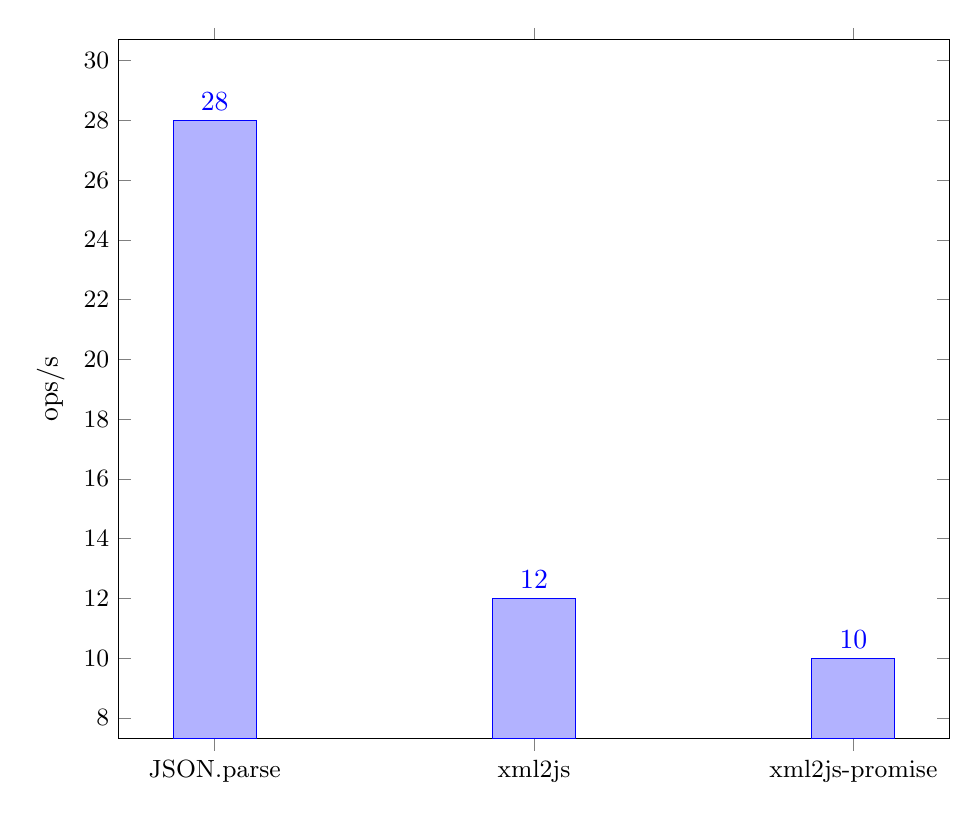
\begin{tikzpicture}
    \begin{axis}
    [
      width=\textwidth,
        bar width=30pt,
        ybar,
        enlargelimits=0.15,
        ylabel={ops/s}, % ylabel 必须在# 符号之前。
        xlabel={},
        symbolic x coords={JSON.parse, xml2js, xml2js-promise}, % 这些是 x 轴坐标的规范。
        xtick=data,
         nodes near coords, % 此命令用于提及特定条形顶部的 y 轴点。
        nodes near coords align={vertical},
        tick label style={font=\small}  
        ]
        \addplot coordinates {(JSON.parse,28) (xml2js,12) (xml2js-promise,10)};
    \end{axis}
  \end{tikzpicture}
    \label{fig:test1}
  \end{minipage}%
  \begin{minipage}{.5\textwidth}
    \centering
  \begin{tikzpicture}
    \begin{axis}
    [
      width=\textwidth,
        bar width=30pt,
        ybar,
        enlargelimits=0.15,
        ylabel={误差率$\pm\%$}, % ylabel 必须在# 符号之前。
        xlabel={},
        symbolic x coords={JSON.parse, xml2js, xml2js-promise}, % 这些是 x 轴坐标的规范。
        xtick=data,
         nodes near coords, % 此命令用于提及特定条形顶部的 y 轴点。
        nodes near coords align={vertical},
        tick label style={font=\small}  
        ]
        \addplot[red, fill=red!40] coordinates {(JSON.parse,4.36) (xml2js,4.16) (xml2js-promise,6.23)};
    \end{axis}
  \end{tikzpicture}
    \label{fig:test2}
  \end{minipage}

  \caption{JSON VS XML 读取解析性能对比}
  \label{fig:json-vs-xml}
\end{figure}

引用可以使用 \verb!\ref! 的方式。

写成如表~\ref{tab:json-vs-xml},将会自动编号。

\section{西红柿炒鸡蛋}

普通文本代码示例:

\begin{lstlisting}[]
  好久不见,你去哪儿啦?

  江湖。

  江湖在什么地方?

  我指给你看………………
\end{lstlisting}


\section{一些语法帮助}

\subsection{枚举示例}

有序号枚举示例:

\begin{enumerate}
  \item 新年快乐
  \item 万事如意
  \item 心想事成
\end{enumerate}

没序号的:

\begin{itemize}
  \item 新年快乐
  \item 万事如意
  \item 心想事成
\end{itemize}

\verb!\backslash! 表示反斜杠,\backslash。


\begin{lstlisting}[]
> 好久不见,你去哪儿啦?
>
> 江湖。
>
> 江湖在什么地方?
>
> 我指给你看………………
\end{lstlisting}

树节点画法:

\begin{figure}[htb]
  \centering
  \begin{minipage}[t]{.4\textwidth}
    \centering
    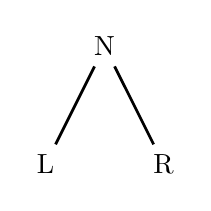
\begin{tikzpicture}[
      line width = 1pt,
      N/.style={draw,circle},
      L/.style={draw,circle, sibling distance=3cm, level distance=1cm},
      R/.style={sibling distance=1.5cm, level distance=0.8cm}]
      \node {N}
      child {node {L}}
      child {node {R}};
    \end{tikzpicture}
  \end{minipage}
  \begin{minipage}[t]{.4\textwidth}
    \centering
    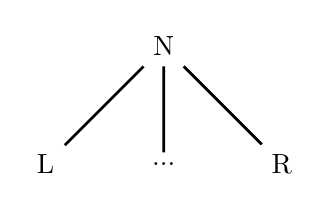
\begin{tikzpicture}[
      line width = 1pt,
      N/.style={draw,circle},
      L/.style={draw,circle, sibling distance=3cm, level distance=1cm},
      R/.style={sibling distance=1.5cm, level distance=0.8cm}]
      \node {N}
      child {node {L}}
      child {node {...}}
      child {node {R}};
    \end{tikzpicture}
  \end{minipage}
  \caption{节点示意图}
  \label{fig:unist-node}
\end{figure}

\begin{figure}[htb]
\centering
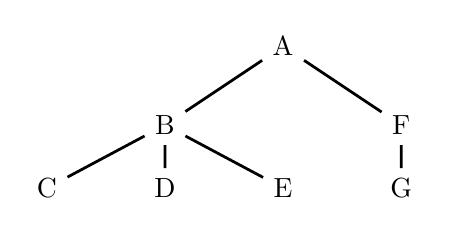
\begin{tikzpicture}[
  line width = 1pt,
  level 1/.style={sibling distance=3cm, level distance=1cm},
  level 2/.style={sibling distance=1.5cm, level distance=0.8cm}]
\node {A}
child {node {B}
  child {node {C}}
  child {node {D}}
  child {node {E}}
}
child {node {F}
  child {node {G}}
};
\end{tikzpicture}
\caption{多节点语法树示意图} \label{fig:unist-tree-example}
\end{figure}


\subsection{实验设计}

...

\subsection{实验结果及分析}

。。。

\section{本章小结}

本章第一节回顾了...

发现还是直接买最方便。

% !TeX root = ../main.tex

\chapter{鸡鸭养殖}

...

\section{画图示例}

TIKZ 画线:

\begin{figure}[htb]
  \centering
  % \subcaptionbox{\label{fig:forward-Kinematic-0}}
  %   {
  %     \begin{tikzpicture}[x=1cm, y=1cm, z=0.6cm]
  %       \draw[line width=2mm] (0,0)  -- (0,2);
  %       \draw[red, line width=1.5mm] (0,2)  -- (0,4.12);
  %       \draw[green, line width=1mm] (0,4.12)  -- (0,5.7);
  %       \draw[blue, line width=0.5mm] (0,5.7)  -- (0, 6.4);
  %     \end{tikzpicture}
  %   }
  \subcaptionbox{\label{fig:forward-Kinematic-1}}
    {
      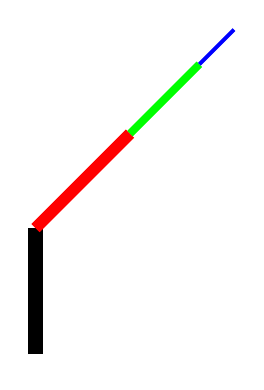
\begin{tikzpicture}[scale=0.8, x=1cm, y=1cm, z=0.6cm]
        \draw[line width=2mm] (0,0)  -- (0,2);
        \draw[red, line width=1.5mm] (0,2)  -- (1.5,3.5);
        \draw[green, line width=1mm] (1.5,3.5)  -- (2.6,4.6);
        \draw[blue, line width=0.5mm] (2.6, 4.6)  -- (3.15, 5.15);
      \end{tikzpicture}
    }
  \subcaptionbox{\label{fig:forward-Kinematics-2}}
    {
      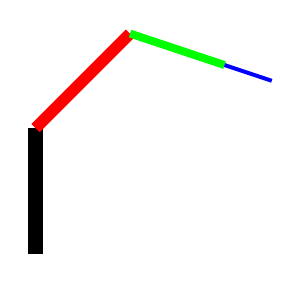
\begin{tikzpicture}[scale=0.8, x=1cm, y=1cm, z=0.6cm]
        \draw[line width=2mm] (0,0)  -- (0,2);
        \draw[red, line width=1.5mm] (0,2)  -- (1.5,3.5);
        \draw[green, line width=1mm] (1.5,3.5)  -- (3,3);
        \draw[blue, line width=0.5mm] (3, 3)  -- (3.75, 2.75);
      \end{tikzpicture}
    }
  \subcaptionbox{\label{fig:forward-Kinematics-3}}
    {
      
\begin{tikzpicture}[scale=0.8, x=1cm, y=1cm, z=0.6cm]
        \draw[line width=2mm] (0,0)  -- (0,2);
        \draw[red, line width=1.5mm] (0,2)  -- (1.5,3.5);
        \draw[green, line width=1mm] (1.5,3.5)  -- (3,3);
        \draw[blue, line width=0.5mm] (3,3)  -- (3.5,2.5);
      \end{tikzpicture}
    }
  \caption{正向动力学}
  \label{fig:forward-Kinematics}
\end{figure}

JavaScript 代码高亮示例:

\begin{lstlisting}[language=JavaScript]
function setup() { // 初始化骨骼结构
  let current = root;
  for(const bone in bones) { // 遍历骨骼(可能存在多个顺序)
    const next = bone.mesh;  current.child = next;  current = next;
  }
}
function draw { // 更新绘制
  while(next) {
    next.update();  next.show();  next = next.child;
  }
}
class Segment { constructor(point, length, angle) {...}  update() { /* 根据父节点更新位置 */ } }
\end{lstlisting}


\subsection{公式示例}

欧拉角转四元数公式:
\begin{equation}
  \begin{aligned}
  \mathbf{q} &= \mathbf{q}_z \mathbf{q}_x \mathbf{q}_y \\
  &={
      \begin{bmatrix}
        \cos(\frac{y}{2})\\0\\0\\\sin(\frac{y}{2})\\
      \end{bmatrix}
    }{
      \begin{bmatrix}
        \cos(\frac{p}{2})\\\sin(\frac{p}{2})\\0\\0\\
      \end{bmatrix}
    }{
      \begin{bmatrix}
        \cos(\frac{r}{2})\\0\\\sin(\frac{r}{2})\\0\\
      \end{bmatrix}
    }\\
  &={
    \begin{bmatrix}
      \cos(\frac{p}{2})\cos(\frac{r}{2})\cos(\frac{y}{2})-\sin(\frac{p}{2})\sin(\frac{r}{2})\sin(\frac{y}{2})\\
      \cos(\frac{p}{2})\cos(\frac{r}{2})\sin(\frac{y}{2})-\cos(\frac{p}{2})\sin(\frac{r}{2})\sin(\frac{y}{2})\\
      \cos(\frac{p}{2})\cos(\frac{r}{2})\sin(\frac{y}{2})+\cos(\frac{p}{2})\sin(\frac{r}{2})\sin(\frac{y}{2})\\
      \cos(\frac{p}{2})\cos(\frac{r}{2})\sin(\frac{y}{2})+\cos(\frac{p}{2})\sin(\frac{r}{2})\sin(\frac{y}{2})\\
    \end{bmatrix}}\\
  \end{aligned}
\end{equation}

四元数转欧拉角时,设 $\mathbf {q} ={\begin{bmatrix}q_{0}&q_{1}&q_{2}&q_{3}\end{bmatrix}}^{T}={\begin{bmatrix}q_{w}&q_{x}&q_{y}&q_{z}\end{bmatrix}}^{T}$,
而求解欧拉角时计算机中的 $arctan$ 与 $arcsin$ 只能获得区间 $(-\frac{\pi}{2},\frac{\pi}{2})$ 的结果,因此使用 $asin$ 替换 $arcsin$,$atan2$ 替换 $arctan$ 函数\cite{babylonZXY},
则:

\begin{equation}
\begin{aligned}
  \begin{bmatrix}
    pitch \\ roll \\ yaw 
  \end{bmatrix}}={
    \begin{bmatrix}
      {\mbox{asin}}(-2(q_z q_y - q_x q_w))\\
      {\mbox{atan2}}(2(q_z q_x + q_y q_w), q_z^2 - q_x^2 - q_y^2 + q_w^2)\\
      {\mbox{atan2}}(2(q_x q_y + q_z q_w), -q_z^2 - q_x^2 + q_y^2 + q_w^2)
    \end{bmatrix}
\end{aligned}
\end{equation}

\subsubsection{插值公式}

\begin{equation}
  y=y_{0}+(x-x_{0}){\frac {y_{1}-y_{0}}{x_{1}-x_{0}}}={\frac {y_{0}(x_{1}-x)+y_{1}(x-x_{0})}{x_{1}-x_{0}}}
\end{equation}


\section{养殖算法}

\subsection{为什么呢}

画立方体:

% draw cube
% https://tex.stackexchange.com/questions/29877/need-help-creating-a-3d-cube-from-a-2d-set-of-nodes-in-tikz
\begin{figure}
  \centering
  \subcaptionbox{切分立方体\label{fig:octree-cube}}
    {
      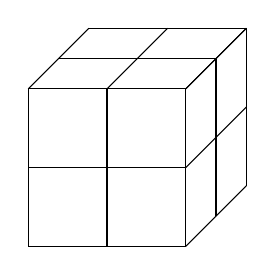
\begin{tikzpicture}
        \foreach \x in{0,...,2}
        {   \draw (0,\x ,2) -- (2,\x ,2);
            \draw (\x ,0,2) -- (\x ,2,2);
            \draw (2,\x ,2) -- (2,\x ,0);
            \draw (\x ,2,2) -- (\x ,2,0);
            \draw (2,0,\x ) -- (2,2,\x );
            \draw (0,2,\x ) -- (2,2,\x );
        }
      \end{tikzpicture}
    }
  \subcaptionbox{对应八叉树\label{fig:octree-tree}}
    {
      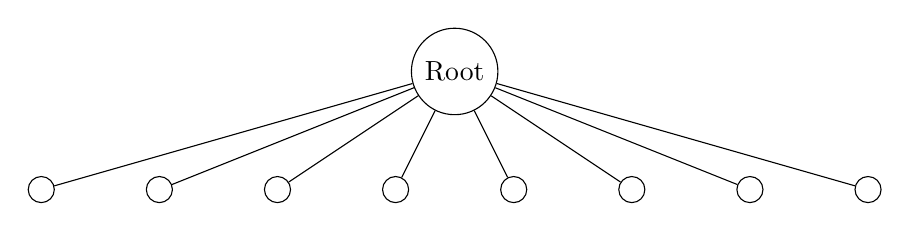
\begin{tikzpicture}
        \tikzstyle{node_style} = [circle,draw=black]
        \node[node_style] {Root}
        child {node[node_style] {}}
        child {node[node_style] {}}
        child {node[node_style] {}}
        child {node[node_style] {}}
        child {node[node_style] {}}
        child {node[node_style] {}}
        child {node[node_style] {}}
        child {node[node_style] {}}
        ;
      \end{tikzpicture}
    }
  \caption{八叉树示例}
  \label{fig:octree}
\end{figure}

放一些看起来高大上的公式。

K-Means 的主要思想是将已知观测集 $(x_1,x_2,...,x_n)$ 划分到 $k$ 个集合($k<=n$),并使每个集合内平方和最小。
即寻找使得下式\eqref{eq:kmeans}最小的聚类 $S_i$($\mu_i$ 是 $S_i$ 中所有点的均值)。
\begin{equation}
  \arg \min_{S_i} \sum_{i=1}^{k} \sum_{x_i \in S_i} (x_i - \mu_i)^2
  \label{eq:kmeans}
\end{equation}

算法实现可主要分为以下两步:分配与更新。

譬如设定存在 $k$ 个初始均值点为 $m_1$,...,$m_k$。

分配:将每个点分配到聚类中,使得集合中的平方和(WCSS)(即平方后的欧式距离)最小。即满足公式\eqref{eq:kmeans_assign}:
\begin{equation}
  S_{i}^{{(t)}}=\left\{x_{p}:\left\|x_{p}-m_{i}^{{(t)}}\right\|^{2}\leq \left\|x_{p}-m_{j}^{{(t)}}\right\|^{2}\forall j,1\leq j\leq k\right\}
  \label{eq:kmeans_assign}
\end{equation}


更新:对于前一步骤得到的每一聚类,重新计算聚类中心(如公式\eqref{eq:kmeans_update}),作为新的均值点。
\begin{equation}
  m_{i}^{{(t+1)}}={\frac  {1}{\left|S_{i}^{{(t)}}\right|}}\sum _{{x_{j}\in S_{i}^{{(t)}}}}x_{j}
  \label{eq:kmeans_update}
\end{equation}


C 代码格式示例:

\begin{lstlisting}[language=c]
  register short *to, *from;
  register count;
  {
    register n = count % 8;
    while (n-- > 0) { 
      *to = *from++;
    }
    n = count / 8;
    if (n == 0) return;     
    do {
      *to = *from++; *to = *from++; *to = *from++; *to = *from++;
      *to = *from++; *to = *from++; *to = *from++; *to = *from++;
    } while (--n > 0)
  }
\end{lstlisting}

三线表:

\begin{table}[h]
  \centering
  \caption{JsPerf (Chrome 84)中循环性能对比}
  \begin{tabular}{p{5cm}p{2cm}}
      \toprule
      \textbf{方法}  & \textbf{Opts/sec} \\
      \midrule
      普通循环 & 165,877  \\
      Duff's Device & 396,801\\
      \bottomrule
  \end{tabular}
  \label{tab:jsperf-efficiency}
\end{table}

\subsubsection{示例图片}

...

多图并列:

\begin{figure}[htbp]
  \centering
  \begin{subfigure}[t]{0.3\textwidth}
  \centering
  \includegraphics[width=.72\textwidth]{yun-kmeans-3.png}
  \caption{K=3}
  \end{subfigure}
  \begin{subfigure}[t]{0.3\textwidth}
  \centering
  \includegraphics[width=.72\textwidth]{yun-kmeans-6.png}
  \caption{K=6}
  \end{subfigure}
  \begin{subfigure}[t]{0.3\textwidth}
  \centering
  \includegraphics[width=.72\textwidth]{yun-kmeans-9.png}
  \caption{K=9}
  \end{subfigure}
  \caption{小云立绘}
  \label{fig:kmeans-png}
\end{figure}


\verb!\href{https://yunyoujun.cn/}{云游君的小站}! 可生成链接\href{https://yunyoujun.cn/}{云游君的小站}。



\section{本章小结}

本章主要介绍...

% !TeX root = ../main.tex

\chapter{系统设计与实现}

本文第三四章中详细介绍了...,
这为最终系统和我财富自由的实现提供了技术基础。...

本章将负责介绍系统的设计与实现,同时这也是本文的最终目的。


\section{设计架构}



pnpm 管理依赖的性能相较 npm、yarn 提升显著,如图~\ref{fig:pnpm-npm-yarn-benchmark}。
\definecolor{pnpm}{HTML}{f1b03d}
\definecolor{npm}{HTML}{be4439}
\definecolor{yarn}{HTML}{458db9}
\definecolor{yarnPnp}{HTML}{5ca9f8}
\begin{figure}
  \centering
  \begin{tikzpicture}
    \begin{axis}[
        xbar=0pt,
        /pgf/bar shift=0pt,
        legend style={
        legend columns=4,
            at={(xticklabel cs:0.5)},
            anchor=north,
            draw=none
        },
        % ytick={pnpm,npm,Yarn,{Yarn PnP}},
        ytick={0,...,4},
        ytick style={draw=none},% <- added
        axis y line*=none,
        axis x line*=bottom,
        legend style={font=\footnotesize},
        label style={font=\footnotesize},
        width=.9\textwidth,
        bar width=4mm,
        yticklabels={
            {pnpm}, 
            {npm}, 
            {Yarn}, 
            {Yarn PnP},
        },
        xlabel={time(s)},
        xmin=0,
        xmax=45,
        area legend,
        y=6mm,
        enlarge y limits={abs=0.625},
        nodes near coords,
        nodes near coords style={text=black},
        every axis plot/.append style={fill},
        tick label style={font=\small},
    ]
      \addplot[fill=pnpm] coordinates {(13,0)};
      \addplot[fill=npm] coordinates {(38.5,1)};
      \addplot[xbar, fill=yarn] coordinates {(16.6,2)};
      \addplot[xbar, fill=yarnPnp] coordinates {(23.6,3)};
    \end{axis}  
  \end{tikzpicture}
  \caption{Monorepo 中 Yarn/pnpm/npm Benchmark}
  \label{fig:pnpm-npm-yarn-benchmark}
\end{figure}

TIKZ 也可以画思维导图,如图~\ref{fig:advjs-modules}。

\begin{figure}[htb]
  \centering
  \begin{tikzpicture}[
    scale=1,
    mindmap, grow cyclic, every node/.style=concept, concept color=purple!20, 
    level 1/.append style={level distance=5cm,sibling angle=90},
    level 2/.append style={level distance=3cm,sibling angle=45},]
    
    \node{ADV.JS}
    child[concept color=green!20] { node {Ecosystem}
      child { node {create-adv 脚手架}}
      child { node {Template 模版示例}}
      child { node {UI 主题}}
    }
    child[concept color=yellow!20] { node {Parser 剧本解析器}
      child { node {AdvScript 语法解析}}
      child { node {unplugin-adv 解析插件}}
      child { node {Vitest 测试}}
      child { node {TypeScript 节点类型定义}}
    }
    child[concept color=blue!20] { node {Editor 编辑器}
      child { node {VRM 编辑器}}
      child { node {剧本编辑器}}
      child { node {VSCode 语法高亮}}
    }
    child[concept color=teal!20] { node {Client 客户端}
      child { node {Adv Ui Components}}
      child { node {Core 核心逻辑}}
      child { node {Store 状态管理}}
      child { node {theme-default}}
    }
    ;
  \end{tikzpicture}
  \caption{模块关系图}
  \label{fig:advjs-modules}
\end{figure}

流程图可以看这里。

\url{https://www.overleaf.com/learn/latex/LaTeX_Graphics_using_TikZ%3A_A_Tutorial_for_Beginners_(Part_3)%E2%80%94Creating_Flowcharts}


\section{客户端开发}

...


\section{系统实现}

各几节介绍一下系统实现的关键技术吧



\section{系统展示}

可以贴点图什么的……

\begin{figure}[htbp]
  \centering
  \includegraphics[width=.5\linewidth]{advjs-black.jpg}
  \caption{测试}
  \label{fig:advjs-debug}
\end{figure}


\section{系统测试与评价}

测试、调查

\section{本章小结}

本章...

% !TeX root = ../main.tex

\chapter{总结与展望}

\section{总结}

本文详细介绍了在...中所做的工作,...

\section{展望}

找不足、展望!



% 其他部分
\backmatter

% \titleformat{\chapter}[hang]{\heiti\sanhao\centering}{}{1em}{}{}
\ctexset{
  chapter = {
    format      = \centering\sffamily\sanhao,
  },
}

% 参考文献
\bibliography{ref/refs}  % 参考文献使用 BibTeX 编译
% \printbibliography       % 参考文献使用 BibLaTeX 编译

% 附录
% \appendix
% !TeX root = ../main.tex

\chapter{附\quad 录}

% \section{图表示例}

% \subsection{图}

% 附录中的图片示例(图~\ref{fig:appendix-figure})。

% \begin{figure}
%   \centering
%   \includegraphics[width=0.6\linewidth]{example-image-a.pdf}
%   \caption{附录中的图片示例}
%   \label{fig:appendix-figure}
% \end{figure}

% \section{相关图表}

% \subsection{表格}

% 从零开始编号
\setcounter{table}{0}
%定义编号格式,在数字序号前加字符“A"

\renewcommand{\thetable}{A.\arabic{table}}

\begin{table}
  \caption{3D 模型格式及作用}
  \begin{tabularx}{\textwidth}{l|XX}
    \toprule
    格式          & 描述  & 优缺点                 \\
    \midrule
    .abc   & 特效工作室主导的通用格式 & 功能强大、通用,但体积大 \\
    .gltf  & 面向 Web 端的格式 & 体积小、跨平台,但功能相对有限  \\
    .fbx & Autodesk 家族通用格式 & 支持动画、兼容广泛,体积与功能介于 abc 与 gltf 之间,通常与 Autodesk 强绑定   \\
    .bvh & BioVision 等设备人物动作捕捉数据 & 通用的人体特征动画文件格式  \\
    .dae & fbx 替代品,基于 XML(Google 地图采用该格式) & 通常需要额外下载软件转换,不够通用  \\
    .stl & 三维打印的通用格式 & 格式简单,只能描述三维物体的几何信息,不支持颜色材质等信息  \\
    .3ds & 三角面静态模型 & 格式简单,难以二次编辑,逐渐被淘汰  \\
    .obj & 静态多边形模型,标准 3D 模型文件格式 & 通用,附带 UV 信息与材质路径,但不包含动画、粒子等信息  \\
    .ply & 静态多边形模型(obj 的升级版),常见于点云扫描 & 改进了 obj 格式所缺少的对任意属性及群组的扩充性  \\
    .psk & Unreal Engine 独有 & 模型带有骨骼动画  \\
    .x3d & 基于 XML 的 Web3D 标记语言,ISO 认证的国际标准 & VRML 标准的升级版本,但制作工具和开发环境相对落后,占有率不高  \\
    .dxf & CAD 通用格式 & 矢量作图通用标准  \\
    \bottomrule
  \end{tabularx}
  \label{tab:3d-model-format}
\end{table}

\begin{table}
  \centering
  \caption{人体模型骨骼索引}
  \begin{tabular}{ll|ll}
    \toprule
    骨骼索引名        & 描述                       & 骨骼索引名        & 描述 \\
    \midrule
    hips &  臀部 & leftThumbProximal &  左拇指根部 \\
    leftUpperLeg &  左大腿 & leftThumbIntermediate &  左拇指中部 \\
    rightUpperLeg &  右大腿 & leftThumbDistal &  左拇指端部 \\
    leftLowerLeg &  左小腿 & leftIndexProximal &  左食指根部 \\
    rightLowerLeg &  右小腿 & leftIndexIntermediate &  左食指中部 \\
    leftFoot &  左脚 & leftIndexDistal &  左食指端部 \\
    rightFoot &  右脚 & leftMiddleProximal &  左中指根部 \\
    spine &  脊柱 & leftMiddleIntermediate &  左中指中部 \\
    chest &  胸部 & leftMiddleDistal &  左中指端部 \\
    neck &  脖子 & leftRingProximal &  左无名指根部 \\
    head &  头部 & leftRingIntermediate &  左无名指中部 \\
    leftShoulder &  左肩 & leftRingDistal &  左无名指端部 \\
    rightShoulder &  右肩 & leftLittleProximal &  左小指根部 \\
    leftUpperArm &  左大臂 & leftLittleIntermediate &  左小指中部 \\
    rightUpperArm &  右大臂 & leftLittleDistal &  左小指端部 \\
    leftLowerArm &  左小臂 & rightThumbProximal &  右拇指根部 \\
    rightLowerArm &  右小臂 & rightThumbIntermediate &  右拇指中部 \\
    leftHand &  左手 & rightThumbDistal &  右拇指端部 \\
    rightHand &  右手 & rightIndexProximal &  右食指根部 \\
    leftToes &  左脚趾 & rightIndexIntermediate &  右食指中部 \\
    rightToes &  右脚趾 & rightIndexDistal &  右食指端部 \\
    leftEye &  左眼 & rightMiddleProximal &  右中指根部 \\
    rightEye &  右眼 & rightMiddleIntermediate &  右中指中部 \\
    jaw &  下颌 & rightMiddleDistal &  右中指端部 \\
    lastBone &  最后一块骨骼索引分隔符 & rightRingProximal &  右无名指根部 \\
    upperChest &  上胸膛 & rightRingIntermediate &  右无名指中部 \\
    rightRingDistal &  右无名指端部 & rightLittleIntermediate &  右小指中部 \\
    rightLittleProximal &  右小指根部 & rightLittleDistal &  右小指端部 \\
    \bottomrule
  \end{tabular}
  \label{tab:human-body-bones}
\end{table}

% 符号对照表
% !TeX root = ../main.tex

\begin{denotation}[3cm]
  \item[AVG/ADV] 文字冒险游戏(Adventure Game)
  \item[AST] 抽象语法树(Abstract Syntax Tree)
  \item[FSM] 有限状态机(Finite-state Machine)
  \item[DFA] 确定有限状态机(Deterministic Finite Automaton)
  \item[BFS] 广度优先搜索(Breadth-First Search)
  \item[DFS] 深度优先搜索(Depth-First-Search)
  \item[PGC] 专业生产内容(Professionally-generated Content)
  \item[UGC] 用户生成内容(User-generated Content)
  \item[VRM] 一种可用于虚拟现实场景的 3D 模型格式(Virtual Reality Model)
  \item[PWA] 渐进式 Web 应用(Progressive Web App)
  \item[Lerp] 线性插值(Linear Interpolation)
  \item[Nlerp] 正规化线性插值(Normalized Linear Interpolation)
  \item[Slerp] 球面线性插值(Spherical Linear Interpolation)
  \item[SPA] 单页应用(Single Page Applications)
  \item[SSR] 服务端渲染(Server-Side Rendering)
  \item[SSG] 静态站点生成(Static Site Generator) 
  \item[FK] 正向动力学(Forward Kinematics)
  \item[IK] 反向动力学(Inverse Kinematics)
  \item[CCDIK] 循环坐标下降反向动力学(Cyclic Coordinate Descent IK)
  \item[FABRIK] 前后延伸反向动力学(Forward And Backward Reaching IK)
\end{denotation}


% 作者简历
% 个人简历、在学期间完成的相关学术成果
% % !TeX root = ../main.tex

\begin{resume}

  % \section*{作者简历}

  % 197× 年 ×× 月 ×× 日出生于四川××县。
  % 1992 年 9 月考入××大学化学系××化学专业,1996 年 7 月本科毕业并获得理学学士学位。
  % 1996 年 9 月免试进入清华大学化学系攻读××化学博士至今。

  % 2019 年 9 月进入中国传媒大学计算机与网络空间安全学院就读计算机应用技术专业数字娱乐与动画技术方向,攻读工学硕士学位。

  % \section*{在学期间所取得的科研成果}

  \subsection*{学术论文}

  \begin{achievements}
    \item 你的论文
  \end{achievements}

  % \subsection*{专利}
  \subsection*{参与软著}

  \begin{achievements}
    \item 你的软著、专利
  \end{achievements}

  \subsection*{参与项目}
  \begin{achievements}
    \item 在学期间参与实验室的项目
  \end{achievements}
\end{resume}


% 致谢
% 盲审时注释掉这里再生成
% !TeX root = ../main.tex

% 盲审时需删掉,在 main.tex 注释掉即可

\begin{acknowledgements}
「反正你还年轻,人生有无限可能。」似乎的确经常从这里或那里看到或听到这样的话。
但我已诞生于此世间足足有四分之一个世纪,同样也几乎走完了人生道路中最重要的四分之一。
时至今日,原本某些柔软的东西也像胡茬一样开始变得硬邦邦的,再也无法逆转。

自三年前进入中国传媒大学读研以来,我的想法与人生目标已发生了许多变化。
我的状态也如同状态机一般不断地从一种状态过渡到另一种状态,可惜其并非确定有限型的。
我的初态与自己的期望相去甚远,但在此期间,却很庆幸地遇到了许多无法预测的可爱的人和事,因此,我决定把它叫做非确定无限状态机。

「假如当时选择了别的道路,会过着不同的大学生活吗?」我不止一次又一次地询问自己,并幻想平行世界中自己的现状。
人生就像是玩文字冒险游戏,做着一个又一个的选择,最后迎来自己所决定的结局。
但与确定有限状态机「确定输入」返回「确定结果」不同,即便同样的初态与输入,时机不同,我也未必拥有相同的结果。
继续倒退,在灰暗的中学时代,我也曾幻想在进入大学后过上如「四叠半神话」中所言的玫瑰色校园生活,与明石相遇、在社团挥洒汗水、精进学业、锻炼身体,未来成为社会栋梁。
但世事难料,我机缘巧合地到了我的母校就读计算机专业,并拖着步伐踩着绊脚石把时光花费在每一条岔路上,最终成为奇形怪状的自己。
而我又抱着类似的希冀与偏执,打了几次挺,来到了如今的母校,并一定程度上再次重复了幻想与放弃的过程。
只是在我以为会望到尽头的研究生生活中,与诸多未曾设想的人与事不期而遇,并走向了人生剧本前几幕中一个还算不错的小结局。

在写代码还是论文时,我似乎总有些洁癖,总是试图寻找更完美的解决方案与排版格式,并在其中蹉跎了大量时间。
也许在几次反复后,项目终究可以收敛于目前可见的最佳方式。
但人生却不会像 ADV 一样可以存档读档,二次修正,从来没有完美的人生与故事,不过正如阿德勒所言,人的可爱之处便在于接受不完美的自己。
过去所有的人与事就如同正向动力学中的骨骼解算,连续的关节依次计算出了如今的自己。
仅仅某个节点的偏差,便可能使端点大相径庭。
我也想不出有限骨骼抵达目前结局的更好解算方式,因此我很感谢在我人生轻小说剧本中出场的关键人物们与此期间的变量。

首先衷心感谢我的引路人XXX老师,这篇论文的顺利完成,离不开她的悉心指导和鼓励。
在实验室的学习生涯和平时的生活中,也从X老师这里学到了很多。
其次则要感谢我的导师XXX老师,平易近人的X老师给了我更多的自由空间。
也十分感谢XXX老师,在游戏策划课上以及实验室例会等,从X老师这里开阔了视野与眼界。
还有在研一研二学习课程时,学院老师们给予的指导。
他们的言传身教将使我终生受益。而我想,这大概也是中传生涯这块骨骼解算的起点。

也感谢实验室的同窗伙伴们X sXX、XXX、XXX、XX、XXX和XXX,和他们共同度过的实验室生活是我难以忘怀的宝贵记忆。
感谢XXX师兄解答了很多写论文时规范经验的问题,感谢XXX、XXX师妹们帮忙校验。
感谢实验室所提供的学习平台与轻松愉快的氛围,也感谢 CBD 中的每一位同学。
感谢过去与现在的室友们,以及同班同学们在校园所交织的故事。
感谢腾讯与支付宝实习期间遇到的同事们,从他们身上我学到了不少开发经验。
感谢开源社区与开源项目们,让我得以快速完成开发工作,并从中学到了许多代码、项目的实践与思考。
感谢相关课题与参考文献的研究学者们,感谢 \LaTeX 与 \thuthesis,让我得以更好地完成论文的撰写与排版工作。

我也想对父母道声谢,在家写论文期间他们为我营造了一个衣食无忧,安静的学习环境,也是他们的支持和鼓励推动着我成为现在的自己。

如今我又将抱着新的期冀启程,幻想玫瑰色的生活,续写有限又无限的可能,直至我的状态机抵达终态。
我不知道到那时骨骼解算的终点在何处,但我想,当我的剧本落下帷幕时,我一定还会回忆并感谢此间登场的变量与关键人物,你们。
  
\end{acknowledgements}
  

% 声明
% \statement
% 将签字扫描后的声明文件 scan-statement.pdf 替换原始页面
% \statement[file=scan-statement.pdf]
% 本科生编译生成的声明页默认不加页脚,插入扫描版时再补上;
% 研究生编译生成时有页眉页脚,插入扫描版时不再重复。
% 也可以手动控制是否加页眉页脚
% \statement[page-style=empty]
% \statement[file=scan-statement.pdf, page-style=plain]



% 指导教师/指导小组学术评语
% \input{data/comments}

% 答辩委员会决议书
% \input{data/resolution}

% 本科生的综合论文训练记录表(扫描版)
% \record{file=scan-record.pdf}

\end{document}
